% RYUON MANUAL
% Copyright (C) 2006 Kengo Ichiki <kichiki@users.sourceforge.net>
% $Id: manual.tex,v 1.2 2006/10/24 20:11:51 kichiki Exp $

\documentclass{book}

\usepackage[dvips]{graphicx}
\usepackage{amsmath}
\usepackage{bm}
\usepackage{times}
\usepackage{txfonts}
\usepackage{mathrsfs}

\begin{document}

\title{RYUON -- a Particle Simulation Suite}
\author{Kengo Ichiki
 \thanks{e-mail: kichiki@users.sourceforge.net}}
\date{\today}

\maketitle

\tableofcontents

\chapter{Introduction}
RYUON is a particle simulation suite,
currently covering Stokesian dynamics method
and hopefully more general many-body problems in the future,
released under the GNU General Public License (see Chapter \ref{chp:GPL}).


My scientific interest is on ``particles in a fluid'' 
or between ``discrete and continuous systems.''
RYU of RYU-ON has meanings of ``grain'' and ``flow'' 
in Japanese and it well fits my interest, the GAP between the two.


I am planning to release the following codes and data:
\begin{itemize}
\item Simulators
  \begin{itemize}
  \item {\tt stokes} (Chapter \ref{chp:stokes}):
    Stokesian dynamics: massless particles in a viscous fluid
  \item 
    Fluidized Beds Simulator: heavy particles in a viscous fluid
    \cite{ichiki1995,ichiki1998}
  \end{itemize}
\item Libraries
  \begin{itemize}
  \item {\tt libstokes} (Chapter \ref{chp:libstokes}):
    library for Stokesian dynamics
    \cite{brady1988a,durlofsky1987a,brady1988b,ichiki2002}
  \item {\tt libiter} (Chapter \ref{chp:libiter}):
    library of iterative solvers for the linear set of equations
    \cite{ichiki2001}
  \item {\tt libexp} (Chapter \ref{chp:libexp}):
    Solver for General Many-Body Problems:
    including electrostatics, gravitational systems,
    elasticity, vortex dynamics, etc
  \item FEM, BEM layer using the above.
  \end{itemize}
\item Data and Details
  \begin{itemize}
  \item {\tt twobody} (Chapter \ref{chp:twobody}):
    The exact solutions for two-body problems in Stokes flows
    \cite{JeffreyOnishi1984,jeffrey1992,jeffrey1993}
  \end{itemize}
\item Utilities: Analysis and Visualization
  \begin{itemize}
  \item Molecular dynamics:
    utility for existing OpenSource Projects such as GROMACS and TINKER
    \cite{IchikiConsta2006}
  \end{itemize}
\end{itemize}




\chapter{{\tt libstokes}:
  Library for Stokesian Dynamics}
\label{chp:libstokes}
\section{API}

\subsection{System Parameters}
System parameters such as the number of particles
are passed to the solver routines by {\tt struct stokes}.

\paragraph{Constructor/Destructor}
\begin{itemize}
\item {\tt stokes\_init ();}
\item {\tt stokes\_free (sys);}
\end{itemize}


\paragraph{Initialize Functions}
\begin{verbatim}
/* set np and nm and allocate the memory for pos[np*3]
 */
void
stokes_set_np (struct stokes * sys,
	       int np, int nm);

void
stokes_set_l (struct stokes * sys,
	      double lx, double ly, double lz);

void
stokes_set_xi (struct stokes * sys,
	       double xi, double cutlim);

double
xi_by_tratio (struct stokes * sys,
	      double tratio);

/* set iter param
 * INPUT
 *   solver : string indicating the solver
 *            sta, sta2, gpb, otmk, or gmres (default)
 *   eps and log10_eps
 *   max (and restart)
 *   debug = 0 : no debug info
 *         = 1 : iteration numbs and residue
 *   out   : FILE * to output debug info.
 */
void
stokes_set_iter (struct stokes * sys,
		 const char * solver,
		 int max,
		 int restart,
		 double eps,
		 int debug,
		 FILE * out);

/* set pos safely by another array
 * INPUT
 *  pos[np*3] :
 */
void
stokes_set_pos (struct stokes * sys,
		const double * pos);
\end{verbatim}

\subsection{NetCDF Interface}
In the library, most data is treated by the pointer
{\tt double *}. Here NetCDF interface for {\tt libstokes}
is prepared for file I/O.

\paragraph{Constructor/Destructor}
The following constructor returns NetCDF id by the returned value.
\begin{itemize}
\item {\tt stokes\_nc\_mob\_f\_init (filename, np);}\\
  activated entries are {\tt f0, x, u}.
\item {\tt stokes\_nc\_mob\_ft\_init (filename, np);}\\
  activated entries are {\tt f0, t0, x, u, o}.
\item {\tt stokes\_nc\_mob\_fts\_init (filename, np);}\\
  activated entries are {\tt f0, t0, e0, x, u, o, s}.
\item {\tt stokes\_nc\_mob\_fix\_f\_init (filename, nm, nf);}\\
  activated entries are {\tt xf0, f0, uf0, x, u, ff}.
\item {\tt stokes\_nc\_mob\_fix\_ft\_init (filename, np);}\\
  activated entries are {\tt xf0, f0, t0, uf0, of0, x, u, o, ff, tf}.
\item {\tt stokes\_nc\_mob\_fix\_fts\_init (filename, np);}\\
  activated entries are {\tt xf0, f0, t0, e0, uf0, of0, ef0,
  x, u, o, s, ff, tf, sf}.
\item {\tt stokes\_nc\_free (nc);}\\
  destructor of NetCDF data structure.
\end{itemize}


\paragraph{Writing Routines}
To set the values to NetCDF data structure,
use the following routines:
\begin{itemize}
\item {\tt stokes\_nc\_set\_?0 (nc, ?0);}\\
    define quantity ``?'' at $t=t_0$,
\item {\tt stokes\_nc\_set\_time (nc, step, time);}\\
    define time $t$ for the step ``{\tt step}'',
\item {\tt stokes\_nc\_set\_? (nc, step, time, ?);}\\
    define quantity ``?'' at $t$ ({\tt step}),
\end{itemize}
where ``?'' is either
{\tt x, u, o, e, f, t, s} (for mobile particles), or
{\tt xf, uf, of, ef, ff, tf, sf} (for fixed particles).



\subsection{Solvers}
Each solver has the name in the form of
\begin{equation}
  {\tt void\quad solve\_\langle type\rangle\_\langle lub\rangle\_ewald\_\langle d\rangle\langle ver\rangle\_\langle mat\rangle(sys,\ givens,\ unknowns);}
\end{equation}

\paragraph{Type of Problem ({\tt type})}
\begin{itemize}
\item ({\tt res}): Resistance Problems\\
  $({\tt u, o, e}) \mapsto ({\tt f, t, s})$
\item ({\tt mob}): Mobility Problems\\
  $({\tt f, t, e}) \mapsto ({\tt u, o, s})$
\item ({\tt mix}): Mobility Problems with Fixed Particles\\
  $({\tt f, t, e, uf, of, ef}) \mapsto ({\tt u, o, s, ff, tf, sf})$
\end{itemize}

\paragraph{Truncation Version ({\tt ver})}
\begin{itemize}
\item ({\tt f}): F version
\item ({\tt ft}): FT version
\item ({\tt fts}): FTS version
\end{itemize}

\paragraph{Lubrication ({\tt lub})}
\begin{itemize}
\item ({\tt lub}): with lubrication
\item (): without lubrication
\end{itemize}

\paragraph{Matrix/$\bm{A}\cdot\bm{x}$ ({\tt mat})}
\begin{itemize}
\item ({\tt matrix}): by matrix procedure
\item (): by $\bm{A}\cdot\bm{x}$ procedure
\end{itemize}

\paragraph{3D/monolayer ({\tt d})}
\begin{itemize}
\item ({\tt 3}): 3D version
\item ({\tt 2}): monolayer version
\end{itemize}


\section{Stokes Flows}
In the following, physical background is explained.

Fluid is described by Navier-Stokes equation
\begin{equation}
  \frac{\partial}{\partial t}
  \Bigl[
    \rho
    \bm{u}
    +
    \left(
      \bm{u}
      \cdot
      \bm{\nabla}
    \right)
    \bm{u}
  \Bigr]
  =
  -
  \bm{\nabla}
  p
  +
  \mu
  \Delta
  \bm{u}
  ,
  \label{eq:navier-stokes}
\end{equation}
where $\bm{u}$ is the fluid velocity,
$p$ is the pressure, $\rho$ is the density,
and $\mu$ is the viscosity.
The differential operator
\begin{equation}
  \bm{\nabla}
  =
  \left[
    \begin{array}{c}
      \partial/\partial x\\
      \partial/\partial y\\
      \partial/\partial z
    \end{array}
  \right]
  ,
\end{equation}
and $\Delta$ is the Laplacian
\begin{equation}
  \Delta
  =
  \bm{\nabla}
  \cdot
  \bm{\nabla}
  =
  \partial^2/\partial x^2
  +
  \partial^2/\partial y^2
  +
  \partial^2/\partial z^2
  .
\end{equation}
This is the fluid equation of motion, in other words,
the momentum balance equation and the counterpart of
Newton's equation of motion $\bm{F} = m\bm{a}$.
Actually, writing the viscous fluid stress by
\begin{equation}
  \bm{\sigma}
  =
  p
  \bm{I}
  +
  \bm{\nabla}\bm{u}
  +
  \Bigl(
  \bm{\nabla}\bm{u}
  \Bigr)^\dagger
  ,
\end{equation}
Navier-Stokes equation (\ref{eq:navier-stokes}) can be written by
the similar equation of motion
\begin{equation}
  \frac{D}{D t}
  \Bigl[
    \rho
    \bm{u}
  \Bigr]
  =
  -
  \bm{\nabla}
  \cdot
  \bm{\sigma}
  .
\end{equation}


The Stokes flows, which is the target of {\tt libstokes},
is where the viscous term in Eq. (\ref{eq:navier-stokes})
is dominating to the inertial term.
The ratio of the magnitude of these two terms are characterized
by a dimensionless number called ``Reynolds number'' $Re$
\begin{equation}
  Re
  :=
  \frac{LU}{\mu}
  ,
\end{equation}
where $L$ and $U$ are characteristic length and velocity.
The Stokes flows are the flow of small Reynolds number.

In the limit $Re\rightarrow 0$,
the governing equation of fluids becomes
\begin{equation}
  \bm{0}
  =
  -
  \bm{\nabla}
  p
  +
  \mu
  \Delta
  \bm{u}
  ,
  \label{eq:stokes}
\end{equation}
which is a linear partial differential equation.
In the following, we are studying fluid motions
governed by Eq. (\ref{eq:stokes})
for incompressible fluid
\begin{equation}
  \bm{\nabla}
  \cdot
  \bm{u}
  =
  0
  .
\end{equation}


\section{Many Body Problem}
In a viscous fluid, objects are dragged by the surrounding fluid.
(Imagine when you are in water pool or the sea.)


\begin{equation}
  \bm{u}
  (\bm{x})
  =
  -
  \frac{1}{8\pi\mu}
  \int_S
  {\rm d}S(\bm{y})\ 
  \bm{J}(\bm{x}-\bm{y})
  \cdot
  \bm{f}(\bm{y})
  .
  \label{eq:stokes-integral}
\end{equation}

Boundary value problem (Dirichlet problem).

Expanding the integrand in the right-hand side
of Eq. (\ref{eq:stokes-integral},
we have
\begin{equation}
  \bm{u}
  (\bm{x})
  =
  -
  \frac{1}{n!}
  \sum_{n=0}^{\infty}
  \frac{1}{8\pi\mu}
  \Bigl[
    (-)^n
    \bm{\nabla}^n
    \bm{J}
  \Bigr]
  (\bm{x}-\bm{y}_0)
  \odot^n
  \int_S
  {\rm d}S(\bm{y})\ 
  \Bigl[
    \bm{y}
    -
    \bm{y}_0
  \Bigr]^n
  \bm{f}(\bm{y})
  ,
\end{equation}
where we assume that the surface $S$ consists of a single sphere
and $\bm{y}_0$ is its center.

Note that the surface integral in the right-hand side
is a tensor of order $(n+1)$ and
is called the force moment $\mathcal{F}^{(n)}$
\begin{equation}
  \mathcal{F}^{(n)}
  (\bm{y}_0)
  :=
  -
  \int_S
  {\rm d}S(\bm{y})\ 
  \Bigl[
    \bm{y}
    -
    \bm{y}_0
  \Bigr]^n
  \bm{f}(\bm{y})
  ,
\end{equation}
and
\begin{eqnarray}
  \mathcal{F}^{(0)}
  (\bm{y}_0)
  &=&
  \bm{F}
  ,\\
  \mathcal{F}^{(1)}
  (\bm{y}_0)
  &=&
  \bm{\epsilon}
  \cdot
  \bm{T}
  +
  \bm{S}
  .
\end{eqnarray}
Taking the terms up to $n=1$ and substituting the above,
we have an expression\cite{durlofsky1987a}
\begin{equation}
  \bm{u}
  (\bm{x})
  =
  \Bigl(
    1
    +
    \frac{a^2\nabla^2}{6}
  \Bigr)
  \bm{J}
  (\bm{x}-\bm{y}_0)
  \cdot
  \bm{F}
  +
  \bm{R}
  (\bm{x}-\bm{y}_0)
  \cdot
  \bm{T}
  +
  \Bigl(
    1
    +
    \frac{a^2\nabla^2}{10}
  \Bigr)
  \bm{K}
  (\bm{x}-\bm{y}_0)
  \odot^2
  \bm{S}
  ,
\end{equation}
where $\bm{R}$ and $\bm{K}$ are given by
\begin{eqnarray}
  \bm{R}
  &=&
  ,\\
  \bm{K}
  &=&
  .
\end{eqnarray}


Up to this order of expansion,
if we introduce the corresponding velocity moments, that is,
the translational and angular velocity $\bm{U}$ and $\bm{\Omega}$
and the rate of strain tensor $\bm{E}$,
we have the closed linear set of equations
written in the matrix form as
\begin{equation}
  \left[
    \begin{array}{c}
      \bm{U}\\
      \bm{\Omega}\\
      \bm{E}
    \end{array}
  \right]
  =
  \left[
    \begin{array}{ccc}
      \bm{a} & \bm{b} & \bm{g}\\
      \tilde{\bm{b}} & \bm{c} & \bm{h}\\
      \tilde{\bm{g}} & \tilde{h} & \bm{m}
    \end{array}
  \right]
  \cdot
  \left[
    \begin{array}{c}
      \bm{F}\\
      \bm{T}\\
      \bm{S}
    \end{array}
  \right]
  .
  \label{eq:mob-fts}
\end{equation}

From the mathematical property of Eq. (\ref{eq:stokes-integral}),
the whole matrix relating two vectors
$(\bm{U}, \bm{\Omega}, \bm{E})^\dagger$ and
$(\bm{F}, \bm{T}, \bm{S})^\dagger$
should be symmetric.
That is,
\begin{eqnarray}
  a_{ij} &=& a_{ji},\\
  \tilde{b}_{ij} &=& b_{ji},\\
  c_{ij} &=& c_{ji}.
\end{eqnarray}
However, we should note that
once we reduce the elements of vectors,
the symmetry does not hold.
From the definition, the second order tensors $\bm{E}$ and $\bm{S}$
are symmetric and traceless, so that only 5 components
out of $3\times 3$ are independent.
Without the reduction to the independent components,
the linear set of equation becomes ill-defined
and the inverse matrix (with the full components) are not unique.

\paragraph{Question:}
Is there any way of reduction
preserving the symmetric nature?


\section{FTS formulation}
Equation (\ref{eq:mob-fts}) is the famous FTS formulation
derived in the paper of Stokesian dynamics method\cite{durlofsky1987a}.

As shown above, it is natural form in the mathematical sense
that $\bm{U}$, $\bm{\Omega}$ and $\bm{E}$ are in the left-hand side
and $\bm{F}$, $\bm{T}$ and $\bm{S}$ are in the right-hand side.
However, from physical point of view, especially for the rigid particles,
it is not always the case.
For instance, in the resistance problem,
$\bm{U}$ and $\bm{\Omega}$ are given and
$\bm{F}$ and $\bm{T}$ are unknown,
while in the mobility problem,
$\bm{F}$ and $\bm{T}$ are given and
$\bm{U}$ and $\bm{\Omega}$ are unknown.
But from the rigidity of the particles,
$\bm{E}$ is always a given parameter and
$\bm{S}$ is known.
That is, for the mobility problem, it would be the natural form that
\begin{equation}
  \left[
    \begin{array}{c}
      \bm{U}\\
      \bm{\Omega}\\
      \bm{S}
    \end{array}
  \right]
  =
  \bm{M}'
  \cdot
  \left[
    \begin{array}{c}
      \bm{F}\\
      \bm{T}\\
      \bm{E}
    \end{array}
  \right]
  .
\end{equation}
Actually, Kim {\it et al}. take this form
rather than Eq. (\ref{eq:mob-fts}).
But, here, we stick to the FTS form of Eq. (\ref{eq:mob-fts})
as in Jeffrey {\it et al}.
Because the equation is linear,
we can construct the FTE form from FTS as
\begin{eqnarray}
  {\bm{M}'}_{UF}
  &=&
  \bm{M}_{UF}
  -
  \bm{M}_{US}
  \cdot
  \Bigl(
  \bm{M}_{ES}
  \Bigr)^{-1}
  \cdot
  \bm{M}_{EF}
  ,\\
  {\bm{M}'}_{UE}
  &=&
  \bm{M}_{US}
  \cdot
  \Bigl(
    \bm{M}_{ES}
  \Bigr)^{-1}
  ,\\
  {\bm{M}'}_{SF}
  &=&
  -
  \Bigl(
    \bm{M}_{ES}
  \Bigr)^{-1}
  \cdot
  \bm{M}_{EF}
  ,\\
  {\bm{M}'}_{SE}
  &=&
  \Bigl(
    \bm{M}_{ES}
  \Bigr)^{-1}
  ,
\end{eqnarray}
for
\begin{equation}
  \left[
    \begin{array}{c}
      \bm{U}\\
      \bm{S}
    \end{array}
  \right]
  =
  \left[
    \begin{array}{cc}
      {\bm{M}'}_{UF} & {\bm{M}'}_{UE}\\
      {\bm{M}'}_{SF} & {\bm{M}'}_{SE}
    \end{array}
  \right]
  \cdot
  \left[
    \begin{array}{c}
      \bm{F}\\
      \bm{E}
    \end{array}
  \right]
  ,
\end{equation}
where
\begin{equation}
  \left[
    \begin{array}{c}
      \bm{U}\\
      \bm{E}
    \end{array}
  \right]
  =
  \left[
    \begin{array}{cc}
      \bm{M}_{UF} & \bm{M}_{US}\\
      \bm{M}_{EF} & \bm{M}_{ES}
    \end{array}
  \right]
  \cdot
  \left[
    \begin{array}{c}
      \bm{F}\\
      \bm{S}
    \end{array}
  \right]
  .
\end{equation}
Note that, for simplicity, we combine $\bm{\Omega}$ and $\bm{T}$ into
$\bm{U}$ and $\bm{F}$ respectively.


This procedure is exactly applied for the higher orders
of expansions for rigid particles, because not only $\bm{E}$
but the higher order velocity moments should be vanished
(that is, these are always given parameters).


\section{Fixed Particles -- Mixed Problem}
When we are interested in particle dynamics,
the mobility problem is the main target.
However, in several situations, we may want to introduce
fixed particles into the simulation representing some
obstacles or vessel to support other mobile particles.
\cite{ichiki1995}
In those cases, it is not a simple mobility problem but
the mixed problems, that is,
the ``mobility and resistance'' problem.

\begin{equation}
  \left[
    \begin{array}{c}
      \bm{U}^{m}\\
      \bm{E}^{m}\\
      \bm{U}^{f}\\
      \bm{E}^{f}
    \end{array}
  \right]
  =
  \left[
    \begin{array}{cccc}
      \bm{M}_{UF}^{mm} & \bm{M}_{US}^{mm} & \bm{M}_{UF}^{mf} & \bm{M}_{US}^{mf}\\
      \bm{M}_{EF}^{mm} & \bm{M}_{ES}^{mm} & \bm{M}_{EF}^{mf} & \bm{M}_{ES}^{mf}\\
      \bm{M}_{UF}^{fm} & \bm{M}_{US}^{fm} & \bm{M}_{UF}^{ff} & \bm{M}_{US}^{ff}\\
      \bm{M}_{EF}^{fm} & \bm{M}_{ES}^{fm} & \bm{M}_{EF}^{ff} & \bm{M}_{ES}^{ff}\\
    \end{array}
  \right]
  \cdot
  \left[
    \begin{array}{c}
      \bm{F}^{m}\\
      \bm{S}^{m}\\
      \bm{F}^{f}\\
      \bm{S}^{f}
    \end{array}
  \right]
  .
\end{equation}



\begin{equation}
  \bm{B}
  \cdot
  \left[
    \begin{array}{c}
      \bm{F}^{m}\\
      \bm{E}^{m}\\
      \bm{U}^{f}\\
      \bm{E}^{f}
    \end{array}
  \right]
  =
  \bm{A}
  \cdot
  \left[
    \begin{array}{c}
      \bm{U}^{m}\\
      \bm{S}^{m}\\
      \bm{F}^{f}\\
      \bm{S}^{f}
    \end{array}
  \right]
  ,
  \label{eq:atimes-gen}
\end{equation}
where given parameters are in the left-hand side
and the unknowns are in the right-hand side.
It is straightforward to obtain the matrices $\bm{A}$ and $\bm{B}$
by $\bm{M}$'s.
\begin{equation}
  \left[
    \begin{array}{cccc}
      -\bm{M}_{UF}^{mm} & \bm{0} & \bm{0} & \bm{0}\\
      -\bm{M}_{EF}^{mm} & \bm{I} & \bm{0} & \bm{0}\\
      -\bm{M}_{UF}^{fm} & \bm{0} & \bm{I} & \bm{0}\\
      -\bm{M}_{EF}^{fm} & \bm{0} & \bm{0} & \bm{I}\\
    \end{array}
  \right]
  \cdot
  \left[
    \begin{array}{c}
      \bm{F}^{m}\\
      \bm{E}^{m}\\
      \bm{U}^{f}\\
      \bm{E}^{f}
    \end{array}
  \right]
  =
  \left[
    \begin{array}{cccc}
      -\bm{I} & \bm{M}_{US}^{mm} & \bm{M}_{UF}^{mf} & \bm{M}_{US}^{mf}\\
      \bm{0}  & \bm{M}_{ES}^{mm} & \bm{M}_{EF}^{mf} & \bm{M}_{ES}^{mf}\\
      \bm{0}  & \bm{M}_{US}^{fm} & \bm{M}_{UF}^{ff} & \bm{M}_{US}^{ff}\\
      \bm{0}  & \bm{M}_{ES}^{fm} & \bm{M}_{EF}^{ff} & \bm{M}_{ES}^{ff}\\
    \end{array}
  \right]
  \cdot
  \left[
    \begin{array}{c}
      \bm{U}^{m}\\
      \bm{S}^{m}\\
      \bm{F}^{f}\\
      \bm{S}^{f}
    \end{array}
  \right]
  .
\end{equation}
Because the matrices are unknown variables,
the generalized form of linear set of equations (\ref{eq:atimes-gen})
can be solved by the standard iterative method
by giving the procedure to calculate $\bm{A}\cdot\bm{x}$
with $\bm{A}$ in (\ref{eq:atimes-gen})
for a given vector $\bm{b} = \bm{B}\cdot\bm{b}'$
appeared in the left-hand side of Eq. (\ref{eq:atimes-gen}).


To reduce the debugging cost (and extra complexity of the code),
the implementation of the scheme in the library {\tt libstokes}
is in this way.\footnote{
  Sometimes, tailor-made implementations for each case,
  that is, resistance, mobility, and mobility/resistance
  (with fixed particles) problems for F, FT, and FTS versions
  (therefore, $3\times 3 = 9$ cases), were faster,
  but it is not drastic at the same time.
  When everything has done and there's nothing to do,
  I'll come back to this point and will revise the codes.}




\section{Lubrication Correction}
One of the innovation done by Stokesian dynamics
\cite{brady1988a,durlofsky1987a,brady1988b}
is the model of lubrication into the system.

\begin{eqnarray}
  \bm{R}
  \simeq
  \left(
    \bm{M}
  \right)^{-1}
  +
  \bm{L}
  .
  \label{eq:res-lub}
\end{eqnarray}

In a straightforward implementation of this lubrication correction,
even in F version, the mobility problem needs twice matrix-inversions.

Here's some trick to prevent the extra matrix-inversion,
which is usually the bottleneck of the calculation
(especially for large systems).
Substituting the resistance matrix (\ref{eq:res-lub})
into the resistance equation and multiplying $\bm{M}$ from the left,
we have the inverse-free matrix equation
\begin{equation}
  \Bigl(
    \bm{I}
    +
    \bm{M}
    \cdot
    \bm{L}
  \Bigr)
  \cdot
  \bm{U}
  =
  \bm{M}
  \cdot
  \bm{F}
  ,
\end{equation}
where $\bm{U}$ and $\bm{F}$ contains all velocity and force moments
for simplicity.
Writing the equation in this form,
we can always apply the generalized linear set of equation
as in Eq. (\ref{eq:atimes-gen}) for any case.


\section{Ewald Summation}
Because of the long-range nature of the Stokeslet $\bm{J}$,
we cannot take a simple cut-off model under the periodic
boundary condition. As in the electrostatic interactions
in solid state physics and molecular dynamics, we should
take Ewald summation technique.

In the Stokes flows, there are mainly two formulations exist:
Hasimoto's formulation\cite{Hasimoto1959}
and Beenakker's formulation\cite{Beenakker1986}.




\chapter{{\tt libiter}: Library of Iterative Solvers}
\label{chp:libiter}
\section{API}
Explain API.

\section{Iterative Method for Dense Matrix}
library of iterative solvers for the linear set of equations
\cite{ichiki2001}


\section{Schemes}
\begin{itemize}
\item Steepest Descent
\item Conjugate Gradient
\item Conjugate Gradient Squared
\item Bi-Conjugate Stabilized
\item Generalized Minimum Residual
\end{itemize}



\chapter{{\tt stokes}: Stokesian Dynamics Simulator}
\label{chp:stokes}

\section{Wrappers}
Currently {\tt libstokes} can be used from the following programming languages:
\begin{itemize}
\item C (native)
\item Python
\item Perl
\item Ruby
\item Guile
\item Octave
\end{itemize}

\section{{\tt xi3}:
  Tuning program for ewald summation parameter}
{\tt xi3} in {\bf RYUON-stokes} package
is a tuning program for ewald summation parameter $\xi$.

For simplicity, here we show the equation for F version.
\begin{eqnarray}
  6\pi\mu a
  \bm{U}^\alpha
  &=&
  \bm{F}^\alpha
  +
  \sum_{\gamma}
  {\sum_{\beta}}'
  \bm{M}(\bm{r}_{\beta\alpha} + \bm{r}_\gamma)
  \cdot\bm{F}^\beta
  \\
  &=&
  \bm{F}^\alpha
  \\
  &&
  +
  \sum_{\gamma}
  {\sum_{\beta\neq\alpha}}'
  \bm{M}^{\rm real}(\bm{r}_{\beta\alpha} + \bm{r}_\gamma)
  \cdot\bm{F}^\beta
  \\
  &&
  +
  \frac{1}{V}
  \sum_{\lambda}
  \sum_{\beta = 1}^{N}
  \cos(\bm{k}_\lambda\cdot\bm{r}_{\beta\alpha})\ 
  \tilde{\bm{M}}^{\rm recip}(\bm{k}_\lambda)
  \cdot\bm{F}^\beta
  \\
  &&
  -
  \bm{M}^{\rm recip}(\bm{r} = \bm{0})
  \cdot\bm{F}^\alpha
  ,
\end{eqnarray}
where $\gamma$ is a index of lattice vector
$\bm{r}_\gamma = (n_x l_x, n_y l_y, n_z l_z)^\dagger$
for arbitrary integers $(n_x, n_y, n_z)$,
$\bm{r}_{\beta\alpha} = \bm{x}^\alpha - \bm{x}^\beta$.
The prime on the summation of particle $\beta$ in real-space lattice sum
means that the self part ($\beta = \alpha$) is excluded
for the primary cell $\bm{r}_{\gamma_0} = \bm{0}$.
The mobility matrix $\bm{M}(\bm{r})$ is so called
Rotne-Prager-Yamakawa tensor given by
\begin{eqnarray}
  \bm{M}(\bm{r})
  &=&
  \frac{3a}{4}
  \left(
    1
    +
    \frac{a^2\nabla^2}{6}
  \right)^2
  \bm{J}(\bm{r})
  \\
  &=&
  \frac{3}{4}
  \left[
  \left(
    \frac{a}{r}
    +
    \frac{a^3}{3r^3}
  \right)
  \bm{I}
  +
  \left(
    \frac{a}{r}
    -
    \frac{a^3}{r^3}
  \right)
  \frac{\bm{rr}}{r^2}
  \right]
  \\
  &=&
  \left(
    \frac{3a}{4}
    +
    \frac{a^3}{4}
    \nabla^2
  \right)
  \left(
    \bm{I}
    \nabla^2
    -
    \bm{\nabla\nabla}
  \right)
  r
  .
\end{eqnarray}
Because it is long-range interaction proportional to $1/r$,
we need to take huge number of periodic images.
The trick of Ewald summation technique is that
using the identity
\begin{equation}
  {\rm erfc}(x) + {\rm erf}(x) \equiv 1,
\end{equation}
we split $\bm{M}(\bm{r})$ into two parts,
$\bm{M}^{\rm real}$ and $\bm{M}^{\rm recip}$ as
\begin{eqnarray}
  \bm{M}^{\rm real}
  &=&
  \left(
    \frac{3a}{4}
    +
    \frac{a^3}{4}
    \nabla^2
  \right)
  \left(
    \bm{I}
    \nabla^2
    -
    \bm{\nabla\nabla}
  \right)
  r\ 
  {\rm erfc} (\xi r),
  \label{eq:xi3-M-real}
  \\
  \bm{M}^{\rm recip}
  &=&
  \left(
    \frac{3a}{4}
    +
    \frac{a^3}{4}
    \nabla^2
  \right)
  \left(
    \bm{I}
    \nabla^2
    -
    \bm{\nabla\nabla}
  \right)
  r\ 
  {\rm erf} (\xi r)
  .
  \label{eq:xi3-M-recip}
\end{eqnarray}
Because the error function ${\rm erfc}(x)$ decays exponentially,
we can truncate the lattice summation of $\gamma$ for $\bm{M}^{\rm real}$
at some point.
Similarly, in reciprocal space, $\tilde{\bm{M}}^{\rm recip}(\bm{k})$
decays exponentially in $k$ so that we can truncate the lattice sum
of $\lambda$ at some point.

Mathematically, the parameter $\xi$ introduced in
Eqs. (\ref{eq:xi3-M-real}) and (\ref{eq:xi3-M-recip})
is arbitrary. It specify how fast $\bm{M}^{\rm real}(\bm{r})$ decays
and how slow $\tilde{\bm{M}}^{\rm recip}(\bm{k})$ decays.
Practically, on the other hand, we can choose the optimal value of $\xi$
so that the calculation time is minimal.


\subsection{Sample Run}
Here is a sample procedure showing how to use {\tt xi3} in practice.
We are looking at the problem of 8 particles at SC lattice sites
in (5, 5, 5) periodic box.
A sample configuration file ({\tt xi3.scm}) is given in the package:
{\small
\begin{verbatim}
; sample set file for xi3
; SC lattice config of 8 particles in (5,5,5) box
; $Id: manual.tex,v 1.2 2006/10/24 20:11:51 kichiki Exp $
(define version    "F")     ; version. "F", "FT", or "FTS"
(define flag-mat   #t)      ; #t => matrix scheme, #f => atimes scheme
(define flag-notbl #f)      ; #t => no-table,      #f => with table

(define np         8)       ; number of particles
(define ewald-eps  1.0e-12) ; cut-off limit for Ewald summation

; lattice vector
(define lattice '(5.0  5.0  5.0))

; configuration of particles
(define x #(
0.0  0.0  0.0
2.5  0.0  0.0
0.0  2.5  0.0
0.0  0.0  2.5
0.0  2.5  2.5
2.5  0.0  2.5
2.5  2.5  0.0
2.5  2.5  2.5
))

; list of time ratio Tr/Tk for Ewald summation (optional)
;(define ewald-trs
;  '(0.1
;    1.0
;    10.0
;    100.0
;    ))
\end{verbatim}
}
Here is a part of the result:
{\small
\begin{verbatim}
# F version table matrix
0.110000 0.245379 22.087 21.575 0.512 1.33163581314065055e-01 2197 125 1713 80
0.121000 0.249308 21.106 20.592 0.514 1.33163581314059309e-01 2197 125 1713 80
0.133100 0.253300 20.812 20.224 0.588 1.33163581314069690e-01 2197 125 1689 92
...
\end{verbatim}
}
Each line of the output consists of 10 columns in this case,
that is, for F version with table.
First 5 columns are the same for any cases;
First and second columns are $R_T$ and $\xi$ (see below in details).
The next 3 are CPU times in milli-seconds
for real space, reciprocal space, and the total
calculations, respectively.
The next column is, for F version, the {\it averaged} velocity
obtained by the calculation (see below in details).
For FT and FTS versions, there are 2 and 3 numbers there.
Next two integers show the lattice points within the range
for real and reciprocal summations. Note that the numbers 
are those in the cubic regions (not spherical). For non-table version
we are taking into account the lattice points within the cubic region
specified by the numbers of lattice points in $x$, $y$, and $z$ directions.
For table version, on the other hand, we apply more complicated 
(and empirical) criteria for the truncation of lattice sum and
roughly speaking this reduce the region from cubic to spherical.
In the case, the final two integers, which are the actual numbers 
of points for real and reciprocal summations we took, are added.



In {\tt xi3} program as well as {\tt libstokes}
library, another parameter $R_T$ instead of $\xi$ is used.
$R_T$ is a rough estimation of CPU time ratio between real and reciprocal
summations and related to $\xi$ as
\begin{equation}
  R_T
  =
  \frac{
    \left(
      l_x l_y l_z
      \xi^3
    \right)^2
  }{\pi^3}   
  =
  \frac{T_{real}}{T_{recip}}
  ,
\end{equation}
where
\begin{equation}
  T_{real}
  \propto
  l_x l_y l_z
  \xi^3
  ,
  \quad
  T_{recip}
  \propto
  k_x k_y k_z
  =
  \frac{\pi^3}{l_x l_y l_z \xi^3}
  .
\end{equation}
\begin{figure}
  \centering
  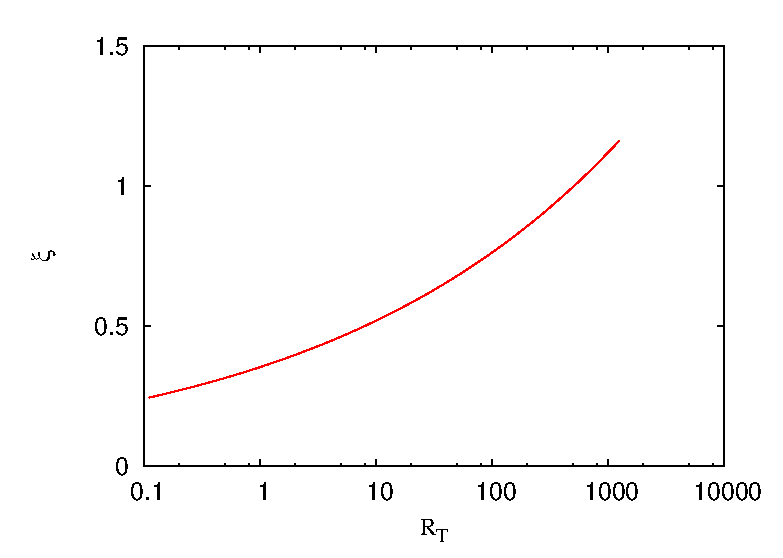
\includegraphics[width=7cm]{figures/FIG-xi3-xi}
  \caption{
    $\xi$ versus $R_T$.
  }
  \label{fig:xi3-xi}
\end{figure}
Figure \ref{fig:xi3-xi} shows $\xi$ vs. $R_T$.
(Those are at the first and second columns in the result file.)
Note that this is implemented in the routine
{\tt xi\_by\_tratio ()}.



Changing $R_T$, the number of lattice points in real and reciprocal
summations are changing: The former is decreasing
and the latter increasing as $R_T$ is increasing.
Because the calculation result is independent of $\xi$ and therefore $R_T$,
we can use this parameter to tune the calculation of the Ewald summation.
That is, we can take a specific value of $\xi$ which minimize
the calculation cost.
This is the whole purpose of {\tt xi3} program.
Figure \ref{fig:xi3-CPU} shows CPU times for real and reciprocal spaces
and the total.
\begin{figure}
  \centering
  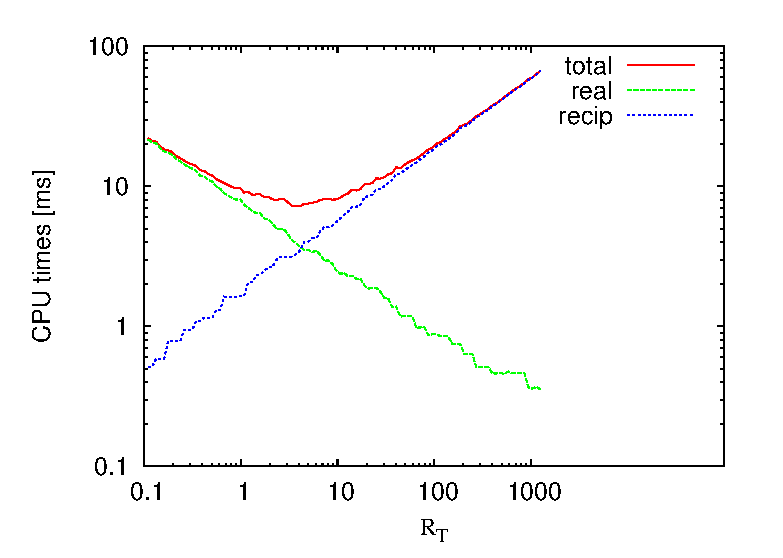
\includegraphics[width=7cm]{figures/FIG-xi3-CPU}
  \caption{
  }
  \label{fig:xi3-CPU}
\end{figure}
As we see, there is an obvious minimum point on the total CPU time.
In this example (for SC lattice of $N=8$ particles in
$(5, 5, 5)$ periodic box),
the minimum is around $R_T\approx 4$.



Previously, I wrote that
the calculation result is independent of $\xi$ and therefore $R_T$.
This is the mathematical conclusion and therefore this is a good 
check for the code:
\begin{quote}
  {\bf The results should be the same for various $\xi$ (and therefore $R_T$).}
\end{quote}
Actually, we truncate the lattice summations at the point where
the term is small enough. The criteria is given by another parameter
{\tt ewald\_eps}.
In this example, we take ${\tt ewald\_eps} = 10^{-12}$.
(Small enough, isn't it?)
In the code of {\tt xi3}, we calculate not physical problems
but the plain $\mathbf{A}\cdot\mathbf{x}$ calculation
for the mobility matrix $\mathbf{A}$ and
a vector $\mathbf{x} = (1,1,\cdots,1)^\dagger$.
The 6th column of the result {\tt xi3} generates
is the average of $\mathbf{A}\cdot\mathbf{x}$, that is,
a kind of averaged velocity. (``a kind of'' means
that the average is taken element-wise rather than particle-wise.)
\begin{figure}
  \centering
  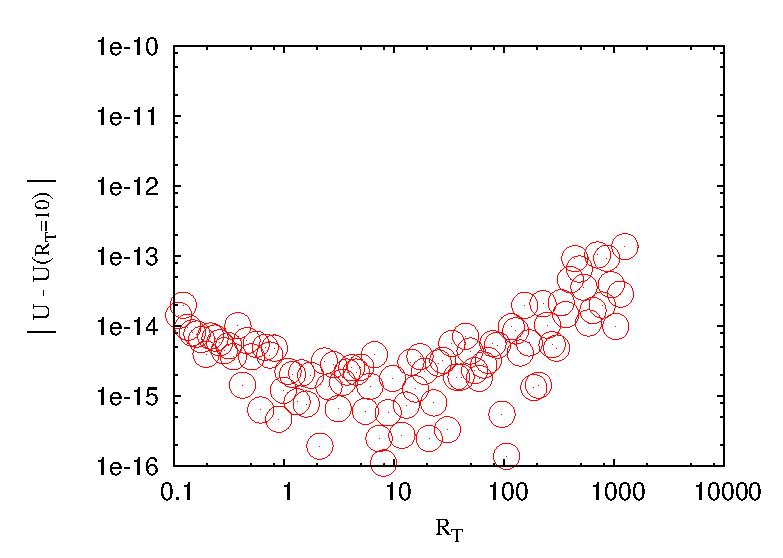
\includegraphics[width=7cm]{figures/FIG-xi3-err}
  \caption{
  }
  \label{fig:xi3-err}
\end{figure}
Figure \ref{fig:xi3-err} shows the calculated results versus $R_T$.
The values in y-axis is the absolute value of the difference
to a point at $R_T \approx 10$, which I just pick to see the 
fluctuations, in other words, the empirical error. (You should 
note that if everything is working good, this approach works,
but otherwise it is not.)
It looks OK.
Actually, my cut-off criteria with {\tt ewald\_eps} might be 
a little hard (because the error is less than 1.0e-13, one order 
lower than expected). But it does not harm and I leave it.


\subsection{Help}
{\small
\begin{verbatim}
$ ./xi3 --help
USAGE
./xi3 init-file
        where init-file is a SCM file (default: xi3.scm)

Parameters in the init-file:
        version    : "F", "FT", or "FTS"
        flag-mat   : #t for matrix-scheme
                   : #f for atimes-scheme
        flag-notbl : calculation scheme for the ewald-summation
                   : #t for no-table
                   : #f for with table
        lattice    : dimensions of the periodic box (list or vector of length 3)
        ewald-eps  : tolerance value for ewald-summation cut-off
        np         : number of particles
        x          : particle configuration (list or vector with length 3*np)
        ewald-trs  : (optional) list of ewald_tr parameters
                   : (list or vector with any length)
\end{verbatim}
}


\chapter{{\tt libexp}:
  Library for Multipole Expansion}
\label{chp:libexp}
We can proceed the expansion beyond the FTS version in principle.

There are several formulations other than the above mentioned
Stokesian dynamics method.
\begin{itemize}
\item Mazur {\it et al}.
\item Sangani {\it et al}.
\end{itemize}
I also developed yet another formalism.\cite{ichiki2002}
The library {\tt libexp} is its implementation.


\section{Multipole Expansion}


\section{Ewald Summation}
Under the periodic boundary,
we can extend the FTS formulation to higher orders.



\section{Fast Multipole Expansion}
Fast Multiple Expansion
\cite{greengard,greengard1987}.




\section{Linear Partial Differential Equations}
Because the formulation is much simpler than others,
the extension to other problems is straightforward.

\begin{itemize}
\item Laplace/Poisson problems (electrostatics)
\item Stokes flows
\item Dynamics of Point Vortices
\item Linear Elastic Problem
\item Gravitational Many Body Problem (Astrophysics)
\item Bubbles in Potential flows
\end{itemize}



\chapter{{\tt twobody}:
  Exact Solutions of Two Rigid Spheres in Stokes Flows}
\label{chp:twobody}

\begin{itemize}
\item Jeffrey and Onishi\cite{JeffreyOnishi1984}
\item Jeffrey\cite{jeffrey1992}
\item Jeffrey {\it et al}.\cite{jeffrey1993}
\end{itemize}



\chapter{Postscript}
Today in science, three fields exist:
theoretical, experimental, and numerical.
The numerical approach is the most recent one
in the scientific research activity.
We should think the procedure in the spirit of scientist.

Imagine a theoretical paper. The author developed some 
theory and wrote the equation down on the paper and published it.
Up to this point, there is no difference from
the activity of novel writers (or whatever).
But one of the strength of science is that
once it is created (or discovered),
the scientific result becomes self-standing
(and sometimes looks trivial).
The point is that anyone can get the same answer
as far as one follows the correct (logical or mathematical)
path, and anyone can test the correctness.
{\it Reproducibility} is the heart of science.


Consider numerical studies.
Someone showed some simulation results by his/her own
developed program. As we know, numerical simulations
are sometimes very sensitive and small changes of 
implementations causes unexpected difference.
How can we feel the same {\it reproducibility}
we can feel on theoretical studies on the numerical stuff?
%
Open source activities fit the needs for the scientific
researches (at least) in terms of numerical methods.
%
We should note that this is not only on the checking processes
on the results, but also for the {\it next} step of the paper.
If we can share the {\it working} code, the progress would
be much faster in any research field. That's what science 
are evolving in the past (mainly on theoretical and 
experimental fields).


This is what I am thinking and why I am releasing my codes.
This is why I took the GNU General Public License
(see Chapter \ref{chp:GPL}), not other licenses.


\newpage

\appendix

{\small
\chapter{The GNU General Public License}
\label{chp:GPL}
\begin{center}
{\parindent 0in

Version 2, June 1991

Copyright \copyright\ 1989, 1991 Free Software Foundation, Inc.

\bigskip

51 Franklin St, Fifth Floor, Boston, MA  02110-1301, USA

\bigskip

Everyone is permitted to copy and distribute verbatim copies
of this license document, but changing it is not allowed.
}

\paragraph{Preamble}
\begin{quote}
The licenses for most software are designed to take away your freedom to
share and change it.  By contrast, the GNU General Public License is
intended to guarantee your freedom to share and change free software---to
make sure the software is free for all its users.  This General Public
License applies to most of the Free Software Foundation's software and to
any other program whose authors commit to using it.  (Some other Free
Software Foundation software is covered by the GNU Library General Public
License instead.)  You can apply it to your programs, too.

When we speak of free software, we are referring to freedom, not price.
Our General Public Licenses are designed to make sure that you have the
freedom to distribute copies of free software (and charge for this service
if you wish), that you receive source code or can get it if you want it,
that you can change the software or use pieces of it in new free programs;
and that you know you can do these things.

To protect your rights, we need to make restrictions that forbid anyone to
deny you these rights or to ask you to surrender the rights.  These
restrictions translate to certain responsibilities for you if you
distribute copies of the software, or if you modify it.

For example, if you distribute copies of such a program, whether gratis or
for a fee, you must give the recipients all the rights that you have.  You
must make sure that they, too, receive or can get the source code.  And
you must show them these terms so they know their rights.

We protect your rights with two steps: (1) copyright the software, and (2)
offer you this license which gives you legal permission to copy,
distribute and/or modify the software.

Also, for each author's protection and ours, we want to make certain that
everyone understands that there is no warranty for this free software.  If
the software is modified by someone else and passed on, we want its
recipients to know that what they have is not the original, so that any
problems introduced by others will not reflect on the original authors'
reputations.

Finally, any free program is threatened constantly by software patents.
We wish to avoid the danger that redistributors of a free program will
individually obtain patent licenses, in effect making the program
proprietary.  To prevent this, we have made it clear that any patent must
be licensed for everyone's free use or not licensed at all.

The precise terms and conditions for copying, distribution and
modification follow.
\end{quote}
\end{center}



\begin{center}
{\Large \sc GNU General Public License
\\\vspace{3mm}Terms and Conditions For Copying, Distribution and Modification}
\end{center}


\begin{enumerate}

\addtocounter{enumi}{-1}

\item 

This License applies to any program or other work which contains a notice
placed by the copyright holder saying it may be distributed under the
terms of this General Public License.  The ``Program'', below, refers to
any such program or work, and a ``work based on the Program'' means either
the Program or any derivative work under copyright law: that is to say, a
work containing the Program or a portion of it, either verbatim or with
modifications and/or translated into another language.  (Hereinafter,
translation is included without limitation in the term ``modification''.)
Each licensee is addressed as ``you''.

Activities other than copying, distribution and modification are not
covered by this License; they are outside its scope.  The act of
running the Program is not restricted, and the output from the Program
is covered only if its contents constitute a work based on the
Program (independent of having been made by running the Program).
Whether that is true depends on what the Program does.

\item You may copy and distribute verbatim copies of the Program's source
  code as you receive it, in any medium, provided that you conspicuously
  and appropriately publish on each copy an appropriate copyright notice
  and disclaimer of warranty; keep intact all the notices that refer to
  this License and to the absence of any warranty; and give any other
  recipients of the Program a copy of this License along with the Program.

You may charge a fee for the physical act of transferring a copy, and you
may at your option offer warranty protection in exchange for a fee.

\item

You may modify your copy or copies of the Program or any portion
of it, thus forming a work based on the Program, and copy and
distribute such modifications or work under the terms of Section 1
above, provided that you also meet all of these conditions:

\begin{enumerate}

\item 

You must cause the modified files to carry prominent notices stating that
you changed the files and the date of any change.

\item

You must cause any work that you distribute or publish, that in
whole or in part contains or is derived from the Program or any
part thereof, to be licensed as a whole at no charge to all third
parties under the terms of this License.

\item
If the modified program normally reads commands interactively
when run, you must cause it, when started running for such
interactive use in the most ordinary way, to print or display an
announcement including an appropriate copyright notice and a
notice that there is no warranty (or else, saying that you provide
a warranty) and that users may redistribute the program under
these conditions, and telling the user how to view a copy of this
License.  (Exception: if the Program itself is interactive but
does not normally print such an announcement, your work based on
the Program is not required to print an announcement.)

\end{enumerate}


These requirements apply to the modified work as a whole.  If
identifiable sections of that work are not derived from the Program,
and can be reasonably considered independent and separate works in
themselves, then this License, and its terms, do not apply to those
sections when you distribute them as separate works.  But when you
distribute the same sections as part of a whole which is a work based
on the Program, the distribution of the whole must be on the terms of
this License, whose permissions for other licensees extend to the
entire whole, and thus to each and every part regardless of who wrote it.

Thus, it is not the intent of this section to claim rights or contest
your rights to work written entirely by you; rather, the intent is to
exercise the right to control the distribution of derivative or
collective works based on the Program.

In addition, mere aggregation of another work not based on the Program
with the Program (or with a work based on the Program) on a volume of
a storage or distribution medium does not bring the other work under
the scope of this License.

\item
You may copy and distribute the Program (or a work based on it,
under Section 2) in object code or executable form under the terms of
Sections 1 and 2 above provided that you also do one of the following:

\begin{enumerate}

\item

Accompany it with the complete corresponding machine-readable
source code, which must be distributed under the terms of Sections
1 and 2 above on a medium customarily used for software interchange; or,

\item

Accompany it with a written offer, valid for at least three
years, to give any third party, for a charge no more than your
cost of physically performing source distribution, a complete
machine-readable copy of the corresponding source code, to be
distributed under the terms of Sections 1 and 2 above on a medium
customarily used for software interchange; or,

\item

Accompany it with the information you received as to the offer
to distribute corresponding source code.  (This alternative is
allowed only for noncommercial distribution and only if you
received the program in object code or executable form with such
an offer, in accord with Subsection b above.)

\end{enumerate}


The source code for a work means the preferred form of the work for
making modifications to it.  For an executable work, complete source
code means all the source code for all modules it contains, plus any
associated interface definition files, plus the scripts used to
control compilation and installation of the executable.  However, as a
special exception, the source code distributed need not include
anything that is normally distributed (in either source or binary
form) with the major components (compiler, kernel, and so on) of the
operating system on which the executable runs, unless that component
itself accompanies the executable.

If distribution of executable or object code is made by offering
access to copy from a designated place, then offering equivalent
access to copy the source code from the same place counts as
distribution of the source code, even though third parties are not
compelled to copy the source along with the object code.

\item
You may not copy, modify, sublicense, or distribute the Program
except as expressly provided under this License.  Any attempt
otherwise to copy, modify, sublicense or distribute the Program is
void, and will automatically terminate your rights under this License.
However, parties who have received copies, or rights, from you under
this License will not have their licenses terminated so long as such
parties remain in full compliance.

\item
You are not required to accept this License, since you have not
signed it.  However, nothing else grants you permission to modify or
distribute the Program or its derivative works.  These actions are
prohibited by law if you do not accept this License.  Therefore, by
modifying or distributing the Program (or any work based on the
Program), you indicate your acceptance of this License to do so, and
all its terms and conditions for copying, distributing or modifying
the Program or works based on it.

\item
Each time you redistribute the Program (or any work based on the
Program), the recipient automatically receives a license from the
original licensor to copy, distribute or modify the Program subject to
these terms and conditions.  You may not impose any further
restrictions on the recipients' exercise of the rights granted herein.
You are not responsible for enforcing compliance by third parties to
this License.

\item
If, as a consequence of a court judgment or allegation of patent
infringement or for any other reason (not limited to patent issues),
conditions are imposed on you (whether by court order, agreement or
otherwise) that contradict the conditions of this License, they do not
excuse you from the conditions of this License.  If you cannot
distribute so as to satisfy simultaneously your obligations under this
License and any other pertinent obligations, then as a consequence you
may not distribute the Program at all.  For example, if a patent
license would not permit royalty-free redistribution of the Program by
all those who receive copies directly or indirectly through you, then
the only way you could satisfy both it and this License would be to
refrain entirely from distribution of the Program.

If any portion of this section is held invalid or unenforceable under
any particular circumstance, the balance of the section is intended to
apply and the section as a whole is intended to apply in other
circumstances.

It is not the purpose of this section to induce you to infringe any
patents or other property right claims or to contest validity of any
such claims; this section has the sole purpose of protecting the
integrity of the free software distribution system, which is
implemented by public license practices.  Many people have made
generous contributions to the wide range of software distributed
through that system in reliance on consistent application of that
system; it is up to the author/donor to decide if he or she is willing
to distribute software through any other system and a licensee cannot
impose that choice.

This section is intended to make thoroughly clear what is believed to
be a consequence of the rest of this License.

\item
If the distribution and/or use of the Program is restricted in
certain countries either by patents or by copyrighted interfaces, the
original copyright holder who places the Program under this License
may add an explicit geographical distribution limitation excluding
those countries, so that distribution is permitted only in or among
countries not thus excluded.  In such case, this License incorporates
the limitation as if written in the body of this License.

\item
The Free Software Foundation may publish revised and/or new versions
of the General Public License from time to time.  Such new versions will
be similar in spirit to the present version, but may differ in detail to
address new problems or concerns.

Each version is given a distinguishing version number.  If the Program
specifies a version number of this License which applies to it and ``any
later version'', you have the option of following the terms and conditions
either of that version or of any later version published by the Free
Software Foundation.  If the Program does not specify a version number of
this License, you may choose any version ever published by the Free Software
Foundation.

\item
If you wish to incorporate parts of the Program into other free
programs whose distribution conditions are different, write to the author
to ask for permission.  For software which is copyrighted by the Free
Software Foundation, write to the Free Software Foundation; we sometimes
make exceptions for this.  Our decision will be guided by the two goals
of preserving the free status of all derivatives of our free software and
of promoting the sharing and reuse of software generally.

\begin{center}
{\Large\sc
No Warranty
}
\end{center}

\item
{\sc Because the program is licensed free of charge, there is no warranty
for the program, to the extent permitted by applicable law.  Except when
otherwise stated in writing the copyright holders and/or other parties
provide the program ``as is'' without warranty of any kind, either expressed
or implied, including, but not limited to, the implied warranties of
merchantability and fitness for a particular purpose.  The entire risk as
to the quality and performance of the program is with you.  Should the
program prove defective, you assume the cost of all necessary servicing,
repair or correction.}

\item
{\sc In no event unless required by applicable law or agreed to in writing
will any copyright holder, or any other party who may modify and/or
redistribute the program as permitted above, be liable to you for damages,
including any general, special, incidental or consequential damages arising
out of the use or inability to use the program (including but not limited
to loss of data or data being rendered inaccurate or losses sustained by
you or third parties or a failure of the program to operate with any other
programs), even if such holder or other party has been advised of the
possibility of such damages.}

\end{enumerate}


\begin{center}
{\Large\sc End of Terms and Conditions}
\end{center}
}


%\bibliographystyle{abbrv}
%\bibliographystyle{alpha}
%\bibliographystyle{apalike}
%\bibliographystyle{ieeetr}
%\bibliographystyle{plain}
\bibliographystyle{siam}
%\bibliographystyle{unsrt}
%\bibliographystyle{prsty}
\bibliography{mine,stokes,fmm}

\end{document}
